\documentclass[10pt,twocolumn,letterpaper]{article}
\usepackage[T1]{fontenc}
\usepackage[review,applications]{wacv}
\usepackage{graphicx,booktabs,amsmath,amssymb,microtype,placeins}
\definecolor{wacvblue}{rgb}{0.13,0.34,0.54}
\usepackage[pagebackref,breaklinks,colorlinks,allcolors=wacvblue]{hyperref}
\def\wacvPaperID{DRAFT}
\def\confName{WACV}
\def\confYear{2027}
\title{Learning Skeleton Representations\\from a Small Collection of Neurological Gait Videos}
\author{Anonymous submission}
\begin{document}
\maketitle

\begin{abstract}
Learning useful descriptions of movement from limited video data could broaden access to quantitative behavioral analysis. We evaluate a compact Skeleton Joint Embedding Predictive Architecture (S-JEPA) on gait videos labeled Normal, multiple sclerosis, or Parkinson's disease. In each split, the model learns from just 24 source videos (45--58 clips) by predicting hidden skeleton features without condition labels. A separate linear classifier then uses its frozen features to predict labels for held-out recordings. Five source-grouped folds cover 88 usable clips from 41 videos. S-JEPA achieves source-weighted macro-F1 of 0.457, exceeding a handcrafted joint-angle Random Forest at 0.325 with mean pose scoring 0.452. The earlier RF implementation, which duplicated an ankle feature, scores 0.411 under the same weighting. During training, the feature-prediction objective decreases while the features retain variation across inputs. The results demonstrate that a compact predictive skeleton model can produce useful features with little study-specific video data. They support a bounded application of representation learning to markerless behavioral analysis: clinical labels are unverified, and matched controls are still needed to measure the added contribution of pretraining and temporal order.
\end{abstract}

\section{Introduction}
Walking provides an observable expression of motor function, making gait a useful subject for behavioral and clinical neuroscience. Multiple sclerosis (MS) can affect joint excursion, stability, and coordination in different combinations across individuals~\cite{filli2018,plotnik2020}. Video-based gait measurements have also been studied in Parkinson's disease (PD)~\cite{shin2021}. These findings motivate the analysis of body movement from ordinary recordings, while leaving a substantial measurement problem: a video contains information about movement alongside the effects of camera position, visibility, and recording conditions.

Markerless pose estimation converts video into trajectories of estimated body landmarks. Studies comparing video-derived gait measurements with reference systems show that this approach can recover useful movement information under specified conditions~\cite{stenum2021,stenum2024}. Once landmarks have been extracted, a common approach is to summarize them through quantities chosen in advance, such as joint angles and their ranges. Learning a representation directly from pose sequences offers another way to describe movement, without specifying every potentially useful relationship between landmarks.

This possibility is particularly relevant when recordings are limited. Self-supervised learning creates a training task from the observations themselves, allowing a model to learn features before condition labels are used. We adapt S-JEPA~\cite{sjepa}, an existing skeleton feature-prediction method, to a small collection of web gait videos. During training, the model predicts features of hidden body regions from the visible parts of a sequence. Its learned feature extractor is then held fixed while a simple classifier is fitted to the collection labels.

Our question is whether this procedure yields useful features on source videos excluded from training. Each model learns from 24 source recordings, and the complete evaluation contains 41 recordings labeled Normal, MS, or PD. The trained features exceed the tested handcrafted joint-angle Random Forest (RF) in the primary source-weighted score, while a mean-pose baseline remains competitive. We contribute a grounded small-data application of predictive skeleton learning and a comparison that makes both the observed advantage and its scope explicit. This work addresses markerless behavioral analysis; it does not include neural recordings or direct neural decoding.

\begin{figure*}[t]
\centering
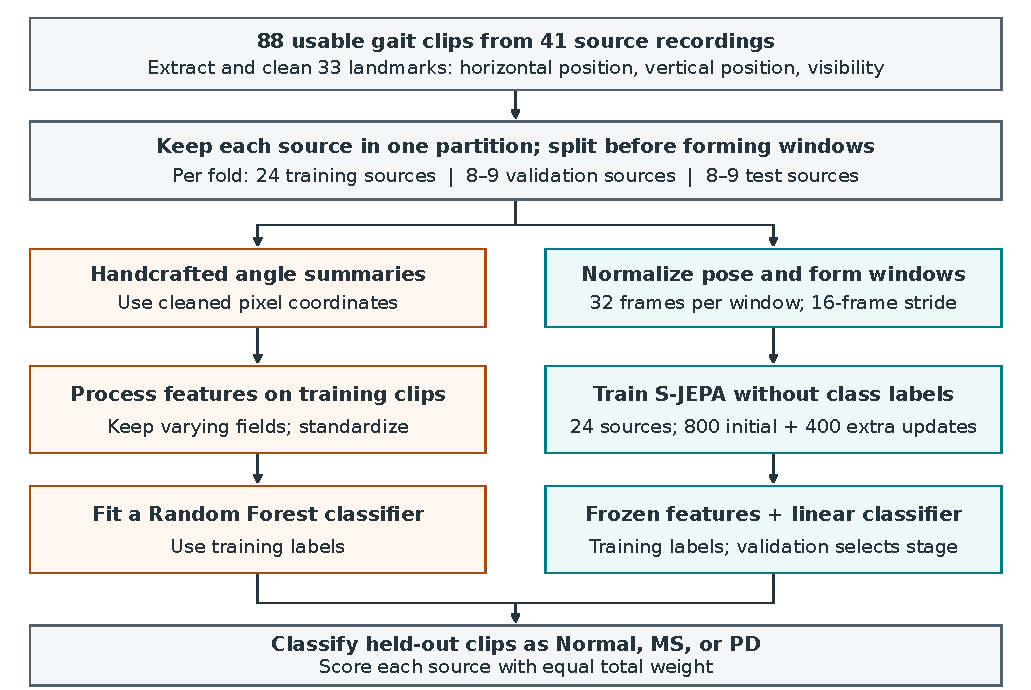
\includegraphics[width=\textwidth]{figures/pipeline.pdf}
\caption{Comparison of learned and handcrafted features. Both branches use the same cleaned pose records and source partitions. The RF computes angles in pixel coordinates; S-JEPA uses body-normalized windows. Only training sources fit features and classifiers, validation selects the S-JEPA stage, and separate test sources provide the reported predictions. The additional mean-pose and visibility baselines are described in the text.}
\label{fig:pipeline}
\end{figure*}

\section{Related work}
\paragraph{Video-based movement measurement.}
Stenum et al. evaluated gait measurements obtained from 2D pose estimation against reference measurements~\cite{stenum2021} and extended the analysis across camera perspectives and clinical populations~\cite{stenum2024}. Shin et al. investigated quantitative gait analysis from single-camera videos of people with PD~\cite{shin2021}. Such work links a defined video-derived quantity to a clinical or biomechanical reference. The present study examines the representation used for label prediction in a web-video collection, where independent diagnoses and reference kinematics are unavailable. Its findings therefore concern the feasibility of the representation and evaluation procedure.

\paragraph{Learning representations for neurological gait.}
Kaur et al. used multi-view video and estimated 3D joints to classify gait strides from people with MS, PD, and matched older adults, with comparisons across participants and walking tasks~\cite{kaur2023}. GaitForeMer pretrained a transformer through motion forecasting together with activity classification, then adapted it to PD gait-impairment severity~\cite{gaitforemer}. These studies establish a close connection between learned skeleton representations and neurological gait analysis. Our study examines a smaller, heterogeneous 2D web-video setting, using a skeleton encoder trained only on the study's training sources and assessed through a frozen-feature classifier. Its contribution is the measured comparison with handcrafted angle features and simple pose summaries under recording-separated evaluation. The datasets, labels, and prediction tasks differ, so the published scores are not direct benchmarks for this experiment.

\paragraph{Learning from skeletons and video.}
SkeletonMAE learns by reconstructing masked skeleton information~\cite{skeletonmae}, and MotionBERT learns motion representations by recovering 3D motion from partial or corrupted 2D observations~\cite{motionbert}. Joint-embedding predictive methods instead predict learned features, as developed for images~\cite{ijepa}, video~\cite{vjepa}, and skeletons~\cite{sjepa}. The original S-JEPA uses motion-aware masking to sample hidden joints. Our compact implementation uses 2D landmarks and detector visibility, with stochastic masks over anatomical regions. The contribution is the application and comparison in a small neurological gait-video collection; the experiment does not establish an algorithmic improvement over the original S-JEPA or a benefit specific to the anatomical mask.



\section{Video collection and pose processing}
Figure~\ref{fig:pipeline} outlines the comparison from cleaned body landmarks to held-out predictions.
The supplied collection contains 91 gait clips from 41 YouTube source videos. The original collection description reports title-based assignment to Normal, MS, and PD, with manual selection of walking segments and cropping where needed to emphasize one person. These are collection labels, without independent clinical verification. Source-video identifiers retained in filenames allow clips from the same recording to be kept together. They do not establish participant identity across recordings.

The processing pipeline uses the pretrained MediaPipe pose landmarker from the BlazePose family~\cite{blazepose}. It retains 33 landmarks with image-plane coordinates and detector visibility; depth is discarded. Frame selection uses integer stride $\max(1,\operatorname{round}(f_{\rm src}/15))$, where $f_{\rm src}$ is the original frame rate. The intended rate is approximately 15 frames per second, but videos are not resampled to a common physical time grid.

Cleaning requires finite horizontal coordinates for all landmarks in at least 30\% of sampled frames and at least eight frames after cleaning. Empty ends are trimmed, missing channels are interpolated, remaining boundary gaps receive the nearest observed value, and a channel with no observations is filled with zero. No maximum interpolation-gap length is imposed. Three clips are excluded, leaving 88 clips and all 41 sources (Table~\ref{tab:data}).

\begin{table}[t]
\centering
\caption{Collection composition. Sources are video recordings, not verified participants. Windows overlap; padded clips contain fewer than 32 cleaned frames.}
\label{tab:data}
\small\setlength{\tabcolsep}{4pt}
\begin{tabular}{lrrrrr}
\toprule
Label & Raw & Usable & Sources & Padded & Windows\\
\midrule
Normal &26&24&16&5&59\\
MS &30&29&13&0&171\\
PD &35&35&12&10&128\\
\midrule
Total &91&88&41&15&358\\
\bottomrule
\end{tabular}
\end{table}

For the learned representation and mean-pose baseline, each frame is centered on the hip midpoint and scaled by the distance between the hip and shoulder midpoints. If $x_{tj}$ is landmark $j$ in frame $t$, and $h_t$ and $s_t$ are those midpoints, then
\begin{equation}
\widetilde{x}_{tj}=\frac{x_{tj}-h_t}{\max(\|s_t-h_t\|_2,10^{-3})}.
\end{equation}
Visibility is unchanged by this spatial normalization. The transformation removes absolute pelvis translation and apparent torso size, so these coordinates are not calibrated measures of walking speed or stride length. The RF branch calculates angles from the cleaned pixel coordinates before this normalization.

Source partitions are fixed before creating 32-frame windows at a stride of 16 frames. Shorter clips are padded by repeating their final frame. The collection provides 358 windows, including 15 padded clips. A window spans roughly two seconds at the nominal sampling rate, with actual duration depending on the source frame rate.

\section{Predictive skeleton learning}
\subsection{Anatomical masking and model structure}
Four consecutive frames for one landmark form an input token containing coordinates and visibility. A window therefore produces eight time blocks and $8\times33=264$ tokens. A new mask hides parts of seven overlapping body regions: head, mouth, left and right arms, trunk, and left and right legs. Each selected region is hidden over one to six consecutive time blocks, with a target of approximately 60\% of the window tokens. The model predicts features for these hidden positions from the remaining context.

The sampler gives additional weight to regions containing any of 12 landmarks: both shoulders, hips, knees, ankles, heels, and foot indices. These landmarks are motivated by the role of lower-limb movement and body coordination in gait~\cite{filli2018,plotnik2020}. Regions containing one of these landmarks receive a 1.5-fold sampling-weight multiplier, with a correction for overlapping membership. Arms receive the same boost through their shoulders. At least one token from this landmark set remains visible somewhere in the window; the rule does not guarantee visible legs in every time block. Supplementary material gives the exact sampling procedure. No separate experiment measured the classification benefit of this anatomical preference.

The context encoder projects tokens into 96-dimensional vectors and adds learned landmark and time-position embeddings. Three transformer layers, each with four attention heads, combine information across visible positions. A two-layer transformer predictor estimates features at hidden positions. The context encoder and predictor contain 402,144 trainable parameters in total, including the learned mask token. A second encoder with the same structure supplies the target features and is updated gradually toward the context encoder using an exponential moving average. The model learns features of missing observations without reconstructing their raw coordinates.

\subsection{Training and representation readout}
The skeleton model starts from random initialization and uses only the training sources in each fold. The upstream pose estimator is already pretrained. All three collection categories are available during encoder training, but their condition labels are not used in the feature-prediction loss. Each batch samples sources uniformly with replacement and then samples a window uniformly within each selected source. This prevents recordings with many windows from dominating encoder training.

The context input receives one geometric transformation per window: rotation within $\pm15^\circ$, scale in $[0.9,1.1]$, translation within $\pm0.1$ normalized units on each axis, and horizontal reflection with probability 0.5. The target input is untransformed. Reflection exchanges left and right landmark slots and visibility values. The stored implementation leaves target-mask indices unchanged during this exchange; the resulting correspondence issue is discussed in Section~\ref{sec:discussion}.

Training compares the predictor's output with features supplied by the target encoder. It subtracts a running feature mean from the target and emphasizes its larger components before calculating a cross-entropy loss, following the centering and sharpening approach of S-JEPA and DINO~\cite{sjepa,dino}. The loss compares distributions over the 96 feature dimensions. These distributions describe learned features, rather than probabilities of the three condition labels. Because the target distribution also changes during training, a decrease in this objective alone does not establish better prediction of a fixed target.

The initial stage uses 800 updates with batches of 32. A second stage continues for 400 updates from the learned weights, restarting the optimizer, feature center, random generators, and learning schedules. Both stages use the same label-free objective. Table~\ref{tab:settings} summarizes the model and optimization settings; the supplementary material records the exact loss and restart procedure.

\begin{table}[t]
\centering
\caption{Model settings used in every fold. The supplementary material records the full recipe and fixed prediction data.}
\label{tab:settings}
\small\setlength{\tabcolsep}{4pt}
\begin{tabular}{lp{1.88in}}
\toprule
Component & Setting\\
\midrule
Window and token & 32 frames; 4 frames per landmark token\\
Encoder & Width 96; 3 layers; 4 attention heads\\
Predictor & Width 96; 2 layers; 4 attention heads\\
Feed-forward layers & Expansion factor 2; dropout 0\\
Training & 800 updates, then 400; batch size 32\\
Optimizer & AdamW; peak rate $10^{-3}$; decay 0.05\\
Learning schedule & 10\% warmup; cosine decay\\
Target update & Momentum from 0.996 toward 1\\
Classification & Frozen features; logistic regression, $C=1$\\
\bottomrule
\end{tabular}
\end{table}

For classification, the selected target encoder is frozen and receives complete, unmasked windows. One fixed readout mask, sampled with seed 0, selects 161 of the 264 output positions, which are averaged to give a 96-number vector per window. Window vectors are then averaged within a clip. Thus, the readout mask selects output features while every input landmark remains available. A scaler fitted on training clips standardizes these features, and a logistic-regression classifier with $C=1$, inverse-frequency class weights, and a 2,000-iteration limit predicts the collection labels. This classifier learns one coefficient per feature for each label. Its training observations are clips, so sources with several clips contribute several observations at this supervised stage.

\section{Evaluation}
\subsection{Keeping source videos separate}
Five outer folds split the 41 source videos while approximately preserving the three label proportions. Within each outer training portion, the first split of a stratified four-fold procedure defines separate training and validation sources. Each fold uses 24 sources for training, 8--9 for validation, and 8--9 for testing. The 24 training sources provide 45--58 clips. No source contributes to more than one partition within a fold, and every usable clip receives exactly one outer-test prediction.

A separate classifier is fitted for each of the two S-JEPA stages. The stage with higher source-weighted validation F1 is selected, retaining the initial stage on a tie. Validation sources are excluded from encoder, scaler, and classifier fitting, and the selected model is not refitted on training plus validation data. Test features are extracted after stage selection. This keeps model selection separate from the assessment on held-out recordings~\cite{varma2006}. All methods use the same partitions and one training seed, 42.

\subsection{Comparison methods}
The handcrafted RF uses summaries of hip, knee, and ankle angles, including side-specific means, bilateral differences, and ranges of movement. Its feature vector has 82 fields, but only 15 angle statistics vary in this collection; the other fields are unpopulated or constant. Columns that do not vary in the training partition are removed. A training-fitted scaler precedes a Random Forest with 100 trees, maximum depth 5, square-root feature subsampling, and balanced class weights. This is a specific lower-limb angle baseline, not a complete set of calibrated clinical gait measurements.

Mean pose averages the normalized horizontal and vertical coordinates of all 33 landmarks across a full clip, giving 66 features and discarding frame order. The visibility baseline uses the mean and standard deviation of each landmark's detector visibility, also giving 66 features. Both use the same independently fitted scaler and logistic-regression recipe as the S-JEPA readout. A majority baseline predicts the most frequent training-clip label. S-JEPA includes visibility as well as coordinates, whereas mean pose uses coordinates alone.

\begin{figure*}[t]
\centering
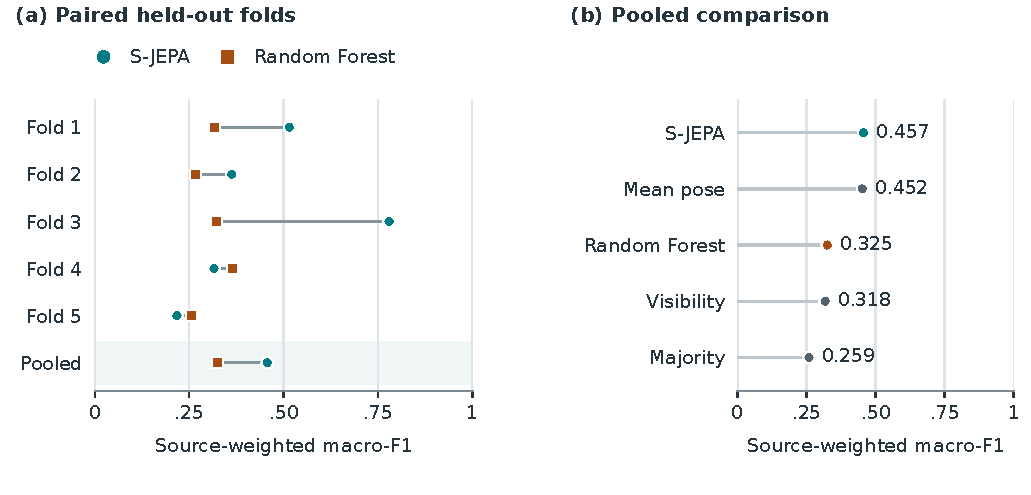
\includegraphics[width=\textwidth]{figures/results.pdf}
\caption{Source-weighted macro-F1 from the corrected evaluation. (a) Straight lines join methods tested on the same held-out sources; they are paired comparisons, not time trends or uncertainty intervals. Fold numbers 1--5 correspond to stored indices 0--4. The pooled row combines all test predictions before scoring. (b) Pooled scores for all five methods. Random Forest denotes the corrected handcrafted angle baseline in both panels.}
\label{fig:results}
\end{figure*}

\subsection{Reporting the comparison}
We report macro-F1, the average of the F1 scores for the three labels. F1 combines how many predictions of a label are correct with how many examples of that label are recovered. The primary score gives each source video equal total weight: a clip from a source with $n_s$ usable clips receives weight $1/n_s$. Weighted prediction counts from all five test folds are pooled before calculating the class scores and their average. This is a clip-level prediction score with equal total source contribution, not classification of one aggregated prediction per source.

We also report a score with equal weight per clip. This comparison matters because one MS source contributes 13 clips. Fold scores describe how results change with the held-out source group; their spread is reported descriptively, without treating the five overlapping training sets as independent repetitions.

The primary results use the complete execution recorded on 9 October 2026 (UTC); the historical RF comparison comes from 21 September 2026. Both use the same fixed dataset and source registry. An earlier execution used the right-ankle range twice in the RF vector instead of separate left and right ranges. We preserve that earlier score as an implementation comparison, rather than silently combining it with the corrected evaluation. No new encoder training was performed for this manuscript revision. The accompanying metric-reproduction packet supplies pseudonymized predictions, source partitions, exact settings, and a dependency-free verification script. It reproduces the reported scores from saved predictions; raw-video access and complete retraining are separate requirements.

\section{Results}
\subsection{Useful features from limited recordings}
The trained S-JEPA representation supports prediction of collection labels on source recordings excluded from training. Its pooled source-weighted macro-F1 is 0.457, compared with 0.325 for the corrected handcrafted RF (Table~\ref{tab:results}). The difference is 0.131 on the 0--1 F1 scale. With equal clip weighting, S-JEPA also exceeds that RF, scoring 0.397 versus 0.321, and correctly classifies 36 of 88 clips compared with 30 for RF. These are observed results from encoders trained on just 24 source videos per fold.

\begin{table}[t]
\centering
\caption{Held-out macro-F1, pooled across all five test folds. Source weighting gives each recording equal total contribution; clip weighting gives each clip equal contribution. The earlier RF row documents the feature implementation change.}
\label{tab:results}
\small\setlength{\tabcolsep}{4pt}
\begin{tabular}{lrrr}
\toprule
Representation & Source & Clip & Correct clips\\
\midrule
S-JEPA + linear classifier &\textbf{0.457}&0.397&36/88\\
Mean pose + linear classifier &0.452&\textbf{0.410}&37/88\\
Joint angles + corrected RF &0.325&0.321&30/88\\
Visibility + linear classifier &0.318&0.318&29/88\\
Majority label &0.259&0.202&23/88\\
\midrule
Earlier RF with duplicate field &0.411&0.397&37/88\\
\bottomrule
\end{tabular}
\end{table}

Mean pose provides a close comparison, scoring 0.452 under source weighting and 0.410 under clip weighting. The S-JEPA margin over mean pose is only 0.005 in the primary score, and mean pose is higher in four of the five individual test folds. The study therefore provides a stronger empirical case for the learned features relative to the tested angle-based RF than for an advantage over a simple full-body pose summary.

The earlier RF implementation scores 0.411 with source weighting. S-JEPA also exceeds that score, by 0.045, while the two methods round to the same clip-weighted F1 of 0.397; the earlier RF is slightly higher before rounding. Correcting the ankle feature changes 12 RF predictions and lowers its score. The two stored executions use the same collection, partitions, and training seed, with identical S-JEPA predicted labels. They are not independent replications of the learned model.

\subsection{Evidence from training}
The saved notebook output for the first training fold reports a decrease in mean feature-prediction loss from 3.858 over the first 50 updates to 1.022 over the last 50 updates of the initial stage. At the same time, mean feature standard deviation rises from 0.154 to 0.526. This diagnostic measures how much each of the 96 features varies across 32 sampled windows, then averages those values; it uses all target-encoder output tokens, whereas classification uses the fixed readout positions. The training objective therefore decreases while the features retain variation across sampled inputs. Since the target distributions also evolve, the loss trend alone cannot establish closer predictor--target agreement. Supplementary material preserves the printed summary and its provenance; a complete numeric learning curve is not retained in the checkpoint.

The training diagnostics and classification results address complementary questions. The diagnostics confirm a functioning optimization process with nonconstant features. The held-out predictions show that a simple classifier can use the resulting features on other source recordings. An identical evaluation of an untrained encoder would be needed to quantify the contribution of pretraining itself.

Continuation lowers the endpoint training loss in every fold, but validation selects it in only two folds. The initial stage is selected for folds 1--3 and continuation for folds 4--5. Feature-prediction loss and downstream label prediction measure different aspects of the representation; validation determines which training stage supplies the reported features.



\subsection{Variation across recordings and labels}
Figure~\ref{fig:results} shows the individual folds alongside the pooled comparison.
S-JEPA exceeds the corrected RF in three of five test folds. Its source-weighted F1 ranges from 0.217 to 0.780, with a mean of 0.438 and standard deviation 0.196. These changes indicate sensitivity to the held-out recordings in this small collection. The result should be read as an observed comparison within the evaluated sources, rather than a guarantee of the same margin in another population.

In raw clip counts, S-JEPA correctly classifies 10 of 24 Normal clips, 8 of 29 MS clips, and 18 of 35 PD clips. It assigns 13 MS clips to PD. The corresponding source-weighted recalls are 39.6\% for Normal, 42.9\% for MS, and 56.9\% for PD; these values give each recording equal total contribution rather than counting clips equally. These errors identify substantial scope for improvement and do not demonstrate reliable discrimination of clinically verified conditions.

\FloatBarrier
\section{Discussion}
\label{sec:discussion}
The main finding is that a compact predictive skeleton model can be trained on a small number of source videos and produce a useful representation for held-out label prediction. Its features are learned from pose observations, without handcrafted angle summaries or condition labels in the encoder objective. A simple classifier fitted to those fixed features exceeds the tested RF in the primary score, including the earlier RF implementation that had a higher observed score. For researchers choosing how to summarize pose recordings, this comparison supports learned full-body features as a useful alternative to the tested lower-limb angle summaries. The competitive mean-pose result also shows why a simple full-body summary deserves a place in such evaluations.

The comparison concerns complete prediction procedures. S-JEPA and RF differ in feature construction and classifier, and only S-JEPA selects between two training stages. The results do not separate those contributions. Mean pose's competitive performance also leaves open how much the S-JEPA features depend on temporal order. The retained experiments do not isolate a gain caused by pretraining or establish which movement information the model uses. Useful representation here means information supporting collection-label prediction; its relationship to specific gait impairments remains to be established.

A known training implementation issue concerns horizontal reflection. Left and right slots are exchanged in the context input while the mask and unreflected target keep their original indices. A physical target joint can consequently appear in the opposite-side context slot. This is a within-example correspondence problem, not mixing of training and test sources. Its impact on learned features was not measured; a matched run with corrected correspondence or reflection disabled is needed. The anatomical weighting likewise remains an untested design hypothesis.

The data also limit clinical interpretation. Labels originate from video descriptions, different source IDs may contain the same participant, and viewpoint or detector behavior may correlate with collection categories. The visibility-only result confirms that coordinate-free detector information supports some label prediction, without identifying its cause. Padding affects five Normal and ten PD clips but no MS clips, and unrestricted interpolation can alter temporal patterns. Framewise normalization removes physical translation and scale, while mean pose and overlapping S-JEPA windows cover frames differently. These observations motivate closer control of sampling and measurement in subsequent studies.

The available collection records do not establish participant consent for secondary health inference, a complete source-media rights assessment, or an ethics-review determination. Public availability alone does not resolve those questions. The study introduces no new participant recruitment and provides no basis for individual clinical decisions; data-use and ethics documentation remain necessary for further release or clinical follow-up.

The most informative next experiment would evaluate a trained encoder and its randomly initialized counterpart under identical partitions and readout settings. Matched frame-order and visibility controls would then help identify what the representation uses. A collection with verified participant identities and diagnoses would allow the resulting features to be evaluated across people and recording sites, and linked to defined movement measurements.

\section{Conclusion}
Predictive skeleton learning produced features that supported gait-video label prediction after training on only 24 source recordings per fold. S-JEPA achieved source-weighted macro-F1 of 0.457, ahead of the corrected handcrafted joint-angle RF at 0.325 and close to mean pose at 0.452. The trained features and their held-out predictions establish a practical starting point for learned pose descriptions in behavioral research. Comparisons with an untrained encoder and clinically verified recordings would clarify how much pretraining contributes and whether the features capture useful neurological movement measurements.

{\small
\bibliographystyle{ieeenat_fullname}
\bibliography{references}
}
\end{document}
